\begin{frame}[label=sep_selection]{Common selection and yearly differences}

\begin{columns}[T]
\column{0.47\textwidth}\small
\textbf{Cut before ML}\par\medskip
\begin{tabular}{ll}\toprule
Variable & Requirement\\\midrule
\var{Bpt} & $15<p_T<50$ GeV\\
\var{By} & $|y|<1.6$\\
\var{BQvalue} & $Q<0.15$ GeV\\\bottomrule
\end{tabular}\par\medskip
Signal: prompt X MC; positive MC weights.\par\medskip
Background: DATA sidebands\par
$(3.80,3.85)\cup(3.89,3.94)$ GeV; unit weights.
\column{0.49\textwidth}\small
\textbf{Yearly difference}\par\medskip
2018: \var{Bchi2Prob}$>0.1$ already imposed upstream.\par\medskip
2023: no additional \var{Bchi2Prob}$>0.1$ requirement in the models shown here.\par\medskip
\textbf{Cut after ML}\par
Each model uses its own Punzi-optimal score, selected with the training sideband range and the total MC sample.
\end{columns}

\end{frame}

\begin{frame}[label=sep_fit3v3]{Combined fit: \var{Btrk1dR}, \var{Btrk2Pt}, \var{Btrk1Pt}}
\begin{columns}[T]
\column{0.49\textwidth}\centering\small\textbf{2018}\quad score $>0.86$\
\par\noindent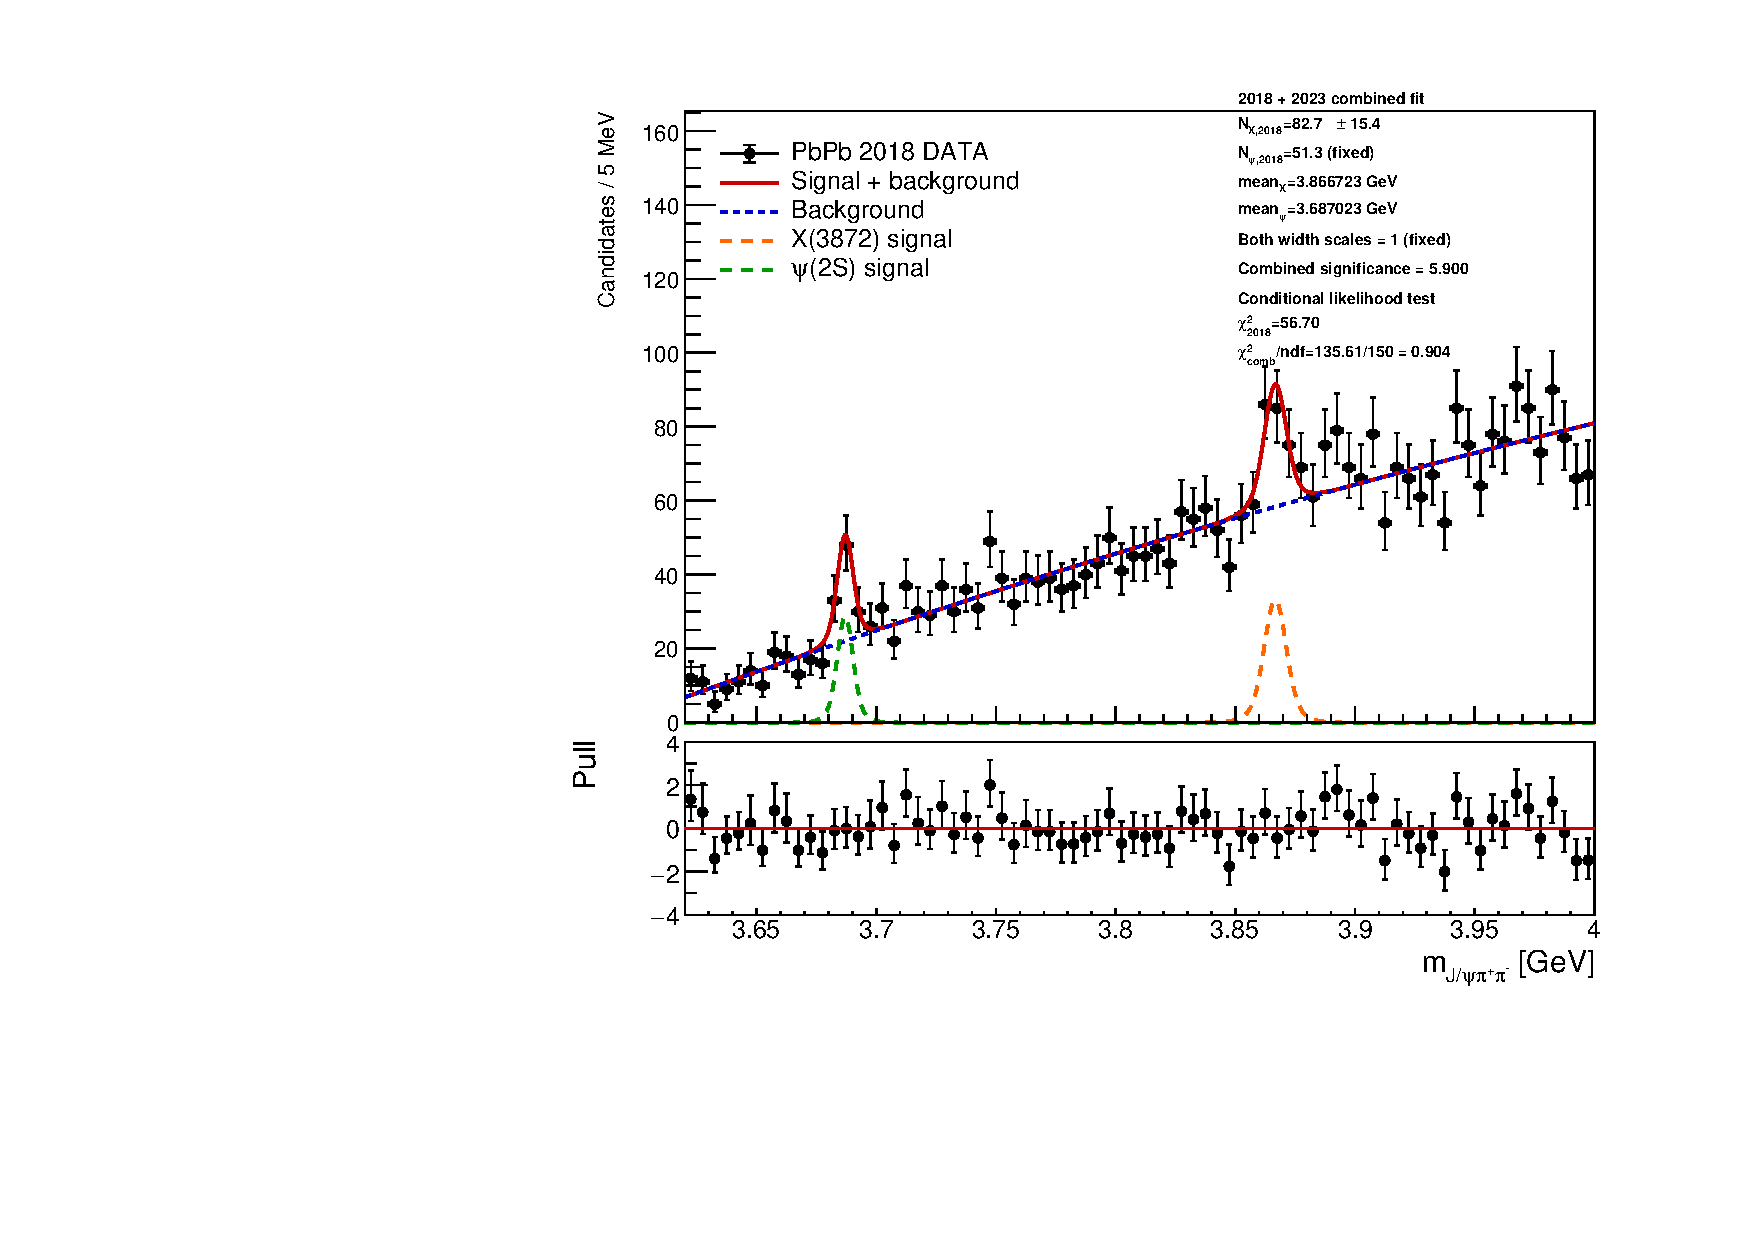
\includegraphics[width=\linewidth,height=0.58\textheight,keepaspectratio]{figures/20260930/3v3/pb18_conditional_fit.pdf}
\column{0.49\textwidth}\centering\small\textbf{2023}\quad score $>0.84$\
\par\noindent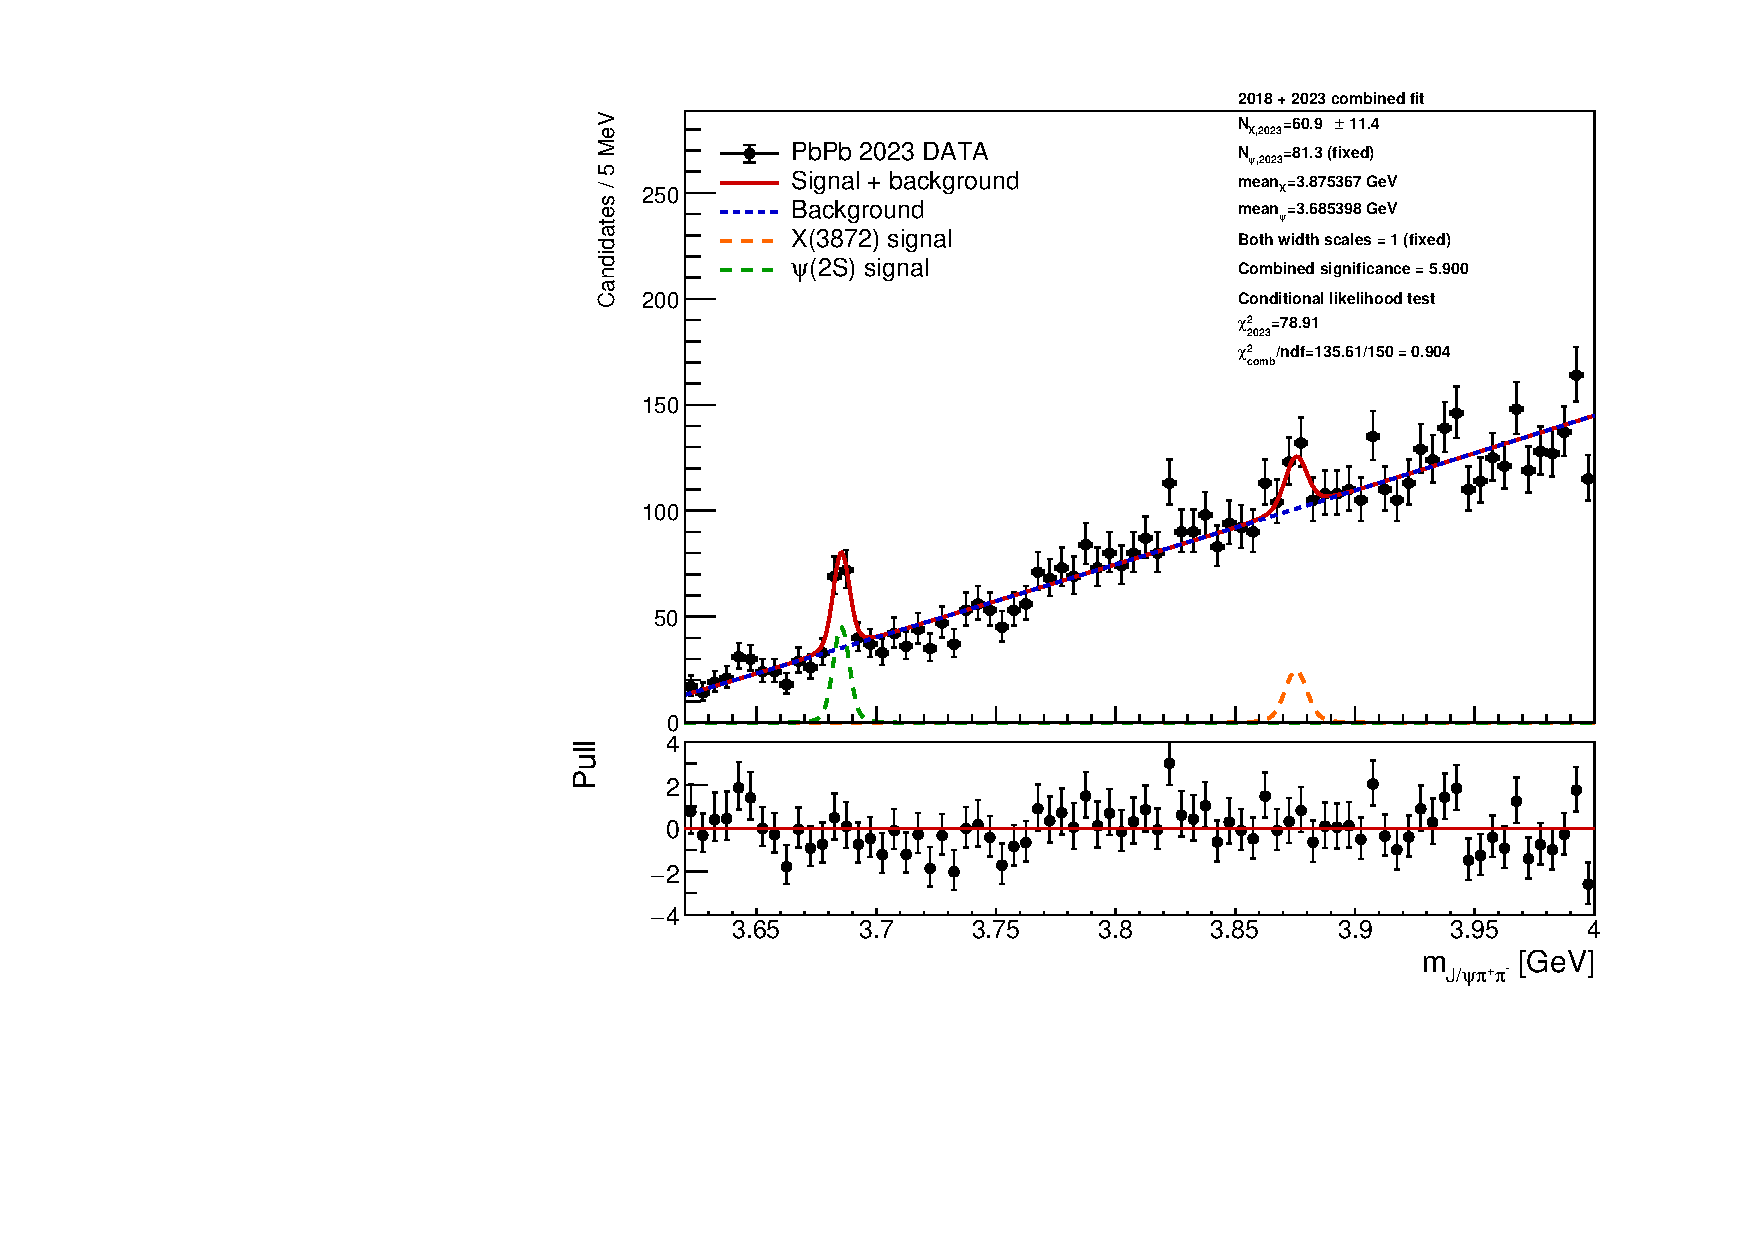
\includegraphics[width=\linewidth,height=0.58\textheight,keepaspectratio]{figures/20260930/3v3/pb23_conditional_fit.pdf}
\end{columns}\small
\textbf{Combined:} $N_X=143.60\pm26.74$; significance $=5.900\sigma$.\par
\textbf{Independent-year reference:} 2018: $5.066\sigma$; 2023: $2.958\sigma$.\par
\textbf{Combined:} $\chi^2/\mathrm{ndf}=0.904$.\par
\caution{MC double-Gaussian widths fixed; 2nd-order Chebyshev background.}

\end{frame}

\begin{frame}[label=sep_fit3v7]{Combined fit: \var{BtrkLeadPt}, \var{BtrkSubPt}, \var{BtrkMaxdR}}
\begin{columns}[T]
\column{0.49\textwidth}\centering\small\textbf{2018}\quad score $>0.86$\
\par\noindent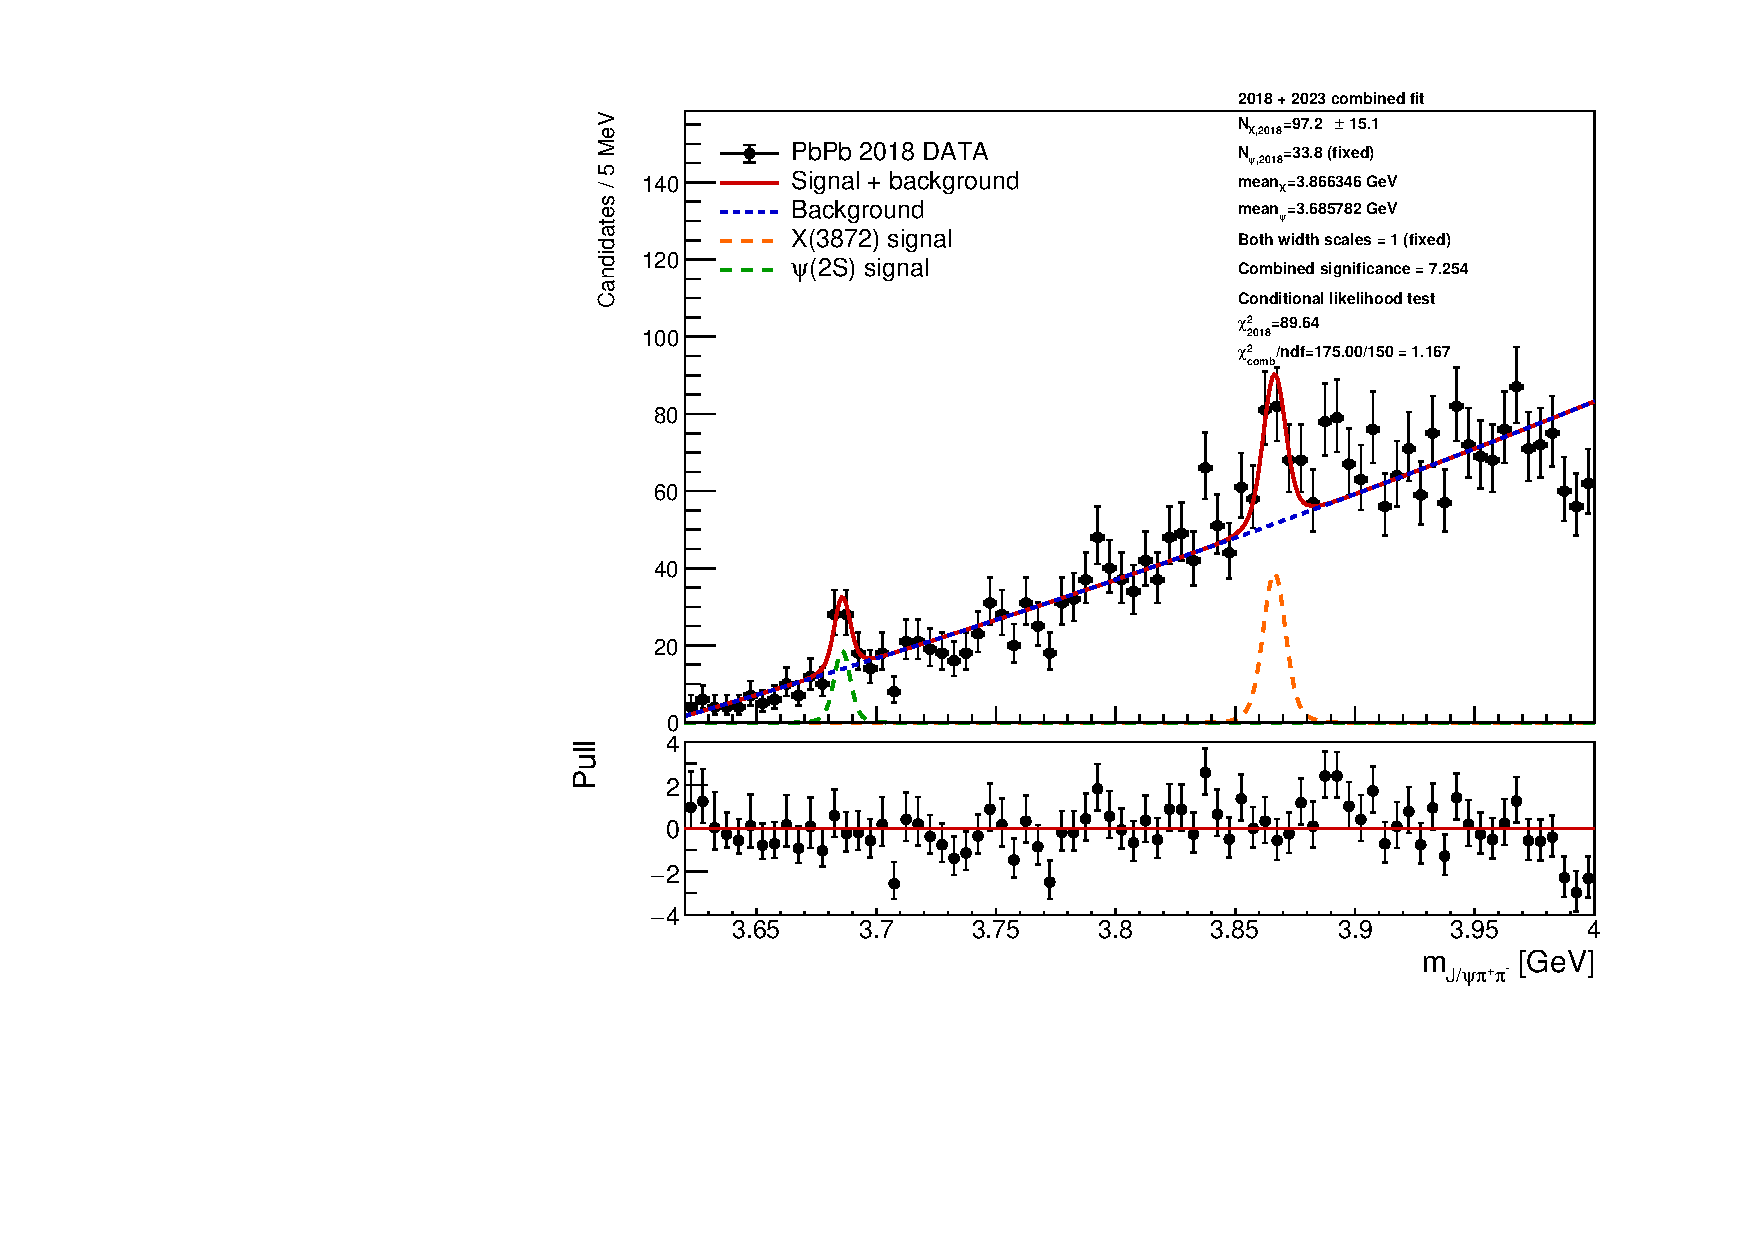
\includegraphics[width=\linewidth,height=0.58\textheight,keepaspectratio]{figures/20260930/3v7/pb18_conditional_fit.pdf}
\column{0.49\textwidth}\centering\small\textbf{2023}\quad score $>0.86$\
\par\noindent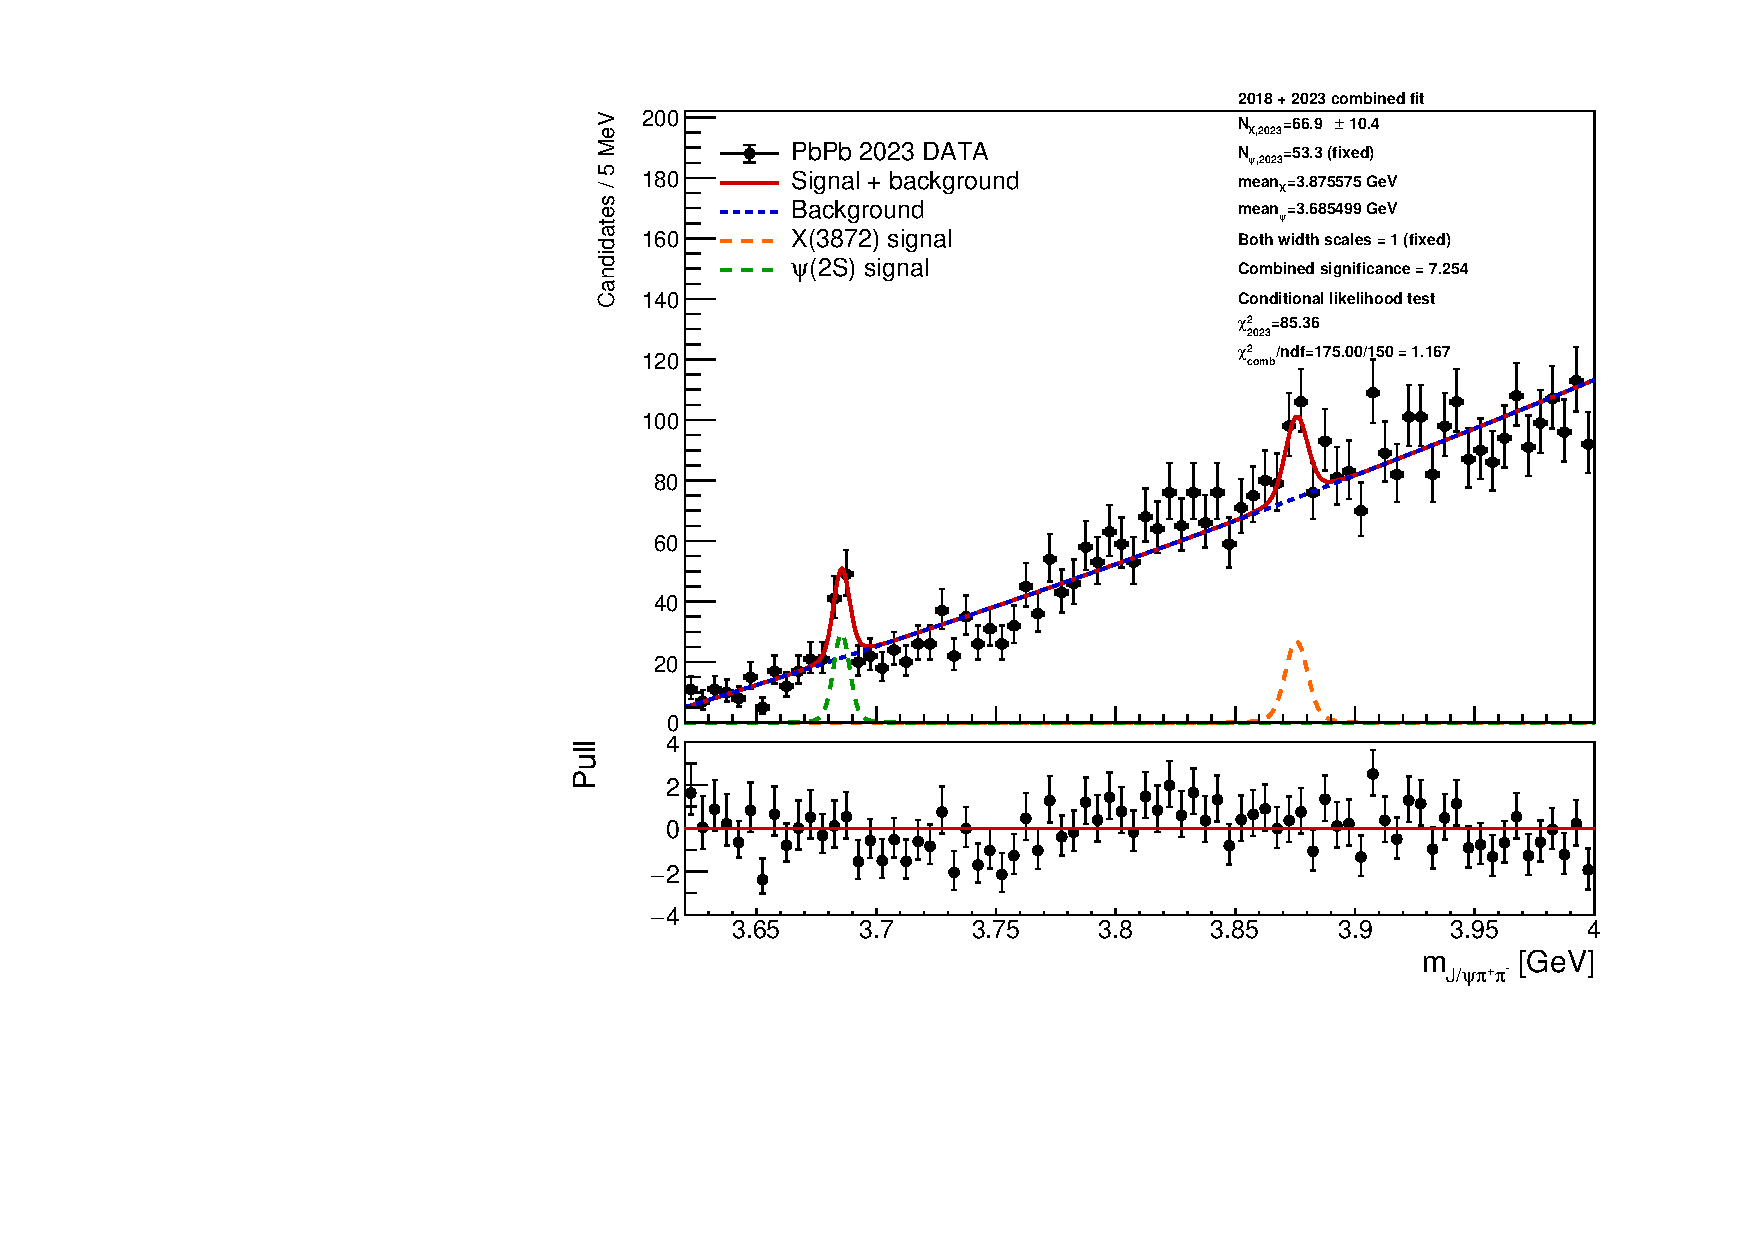
\includegraphics[width=\linewidth,height=0.58\textheight,keepaspectratio]{figures/20260930/3v7/pb23_conditional_fit.pdf}
\end{columns}\small
\textbf{Combined:} $N_X=164.10\pm25.45$; significance $=7.254\sigma$.\par
\textbf{Independent-year reference:} 2018: $6.188\sigma$; 2023: $3.722\sigma$.\par
\textbf{Combined:} $\chi^2/\mathrm{ndf}=1.167$.\par
\caution{MC double-Gaussian widths fixed; 2nd-order Chebyshev background.}

\end{frame}

\begin{frame}[label=sep_summary]{Current preferred candidates}
\small
\begin{center}\begin{tabular}{lrrrrrr}\toprule
Variable set & 3v3 & 3v7 & 9v1 & 5v1 & 3v5 & 3v12\\\midrule
Combined significance [$\sigma$] & 5.900 & 7.254 & 4.703 & 4.410 & 5.573 & 5.961\\\bottomrule
\end{tabular}\end{center}
\begin{columns}[T]
\column{0.57\textwidth}\small
\begin{itemize}\setlength{\itemsep}{2pt}
\item 3v3: \var{Btrk1dR}, \var{Btrk2Pt}, \var{Btrk1Pt}.
\item 3v7: \var{BtrkLeadPt}, \var{BtrkSubPt}, \var{BtrkMaxdR}.
\item 9v1: \var{Bmu1pt}, \var{Bmu1eta}, \var{Bmu2pt}, \var{Bmu2eta}, \var{Btrk2Pt}, \var{BtrkPtimb}, \var{Btrk1dR}, \var{Bujeta}, \var{Btktketa}.
\item 5v1: \var{Bmu1pt}, \var{Bmu2pt}, \var{Btrk2Pt}, \var{BtrkPtimb}, \var{Btrk1dR}.
\item 3v5: \var{Btrk1dR}, \var{Btrk2Pt}, \var{BtrkPtimb}.
\item 3v12: \var{BtrkLeadPt}, \var{BtrkPtimb}, \var{BtrkMaxdR}.
\end{itemize}
\column{0.40\textwidth}\small
\begin{itemize}
\item \textbf{Possible explanation:} for a rare X signal, more variables may make high-dimensional MC mismodelling or overfitting more pronounced.
\medskip
\item \textbf{Current preferred candidates:}\par\smallskip
\var{Btrk1dR}, \var{Btrk2Pt}, \var{Btrk1Pt}\par\smallskip
and\par\smallskip
\var{BtrkLeadPt}, \var{BtrkSubPt}, \var{BtrkMaxdR}.
\end{itemize}
\end{columns}
\end{frame}

\begin{frame}[label=sep_thanks]{\strut}
\centering\vfill
\makebox[\textwidth][c]{%
\begin{beamercolorbox}[wd=0.68\textwidth,sep=1.2em,center,rounded=true,shadow=true]{block body}
{\LARGE\bfseries Thanks for listening!}\par\vspace{1em}
{\large Reporter: Lekai Yao}\par\vspace{0.45em}
{\large 2026.9.30}
\end{beamercolorbox}}
\vfill
\end{frame}

